% arara: lualatex: { synctex: on, shell: off }
% arara: biber
% arara: lualatex: { synctex: on, shell: off }
% arara: sumatrapdf
\documentclass[../main.tex]{subfiles}

% %Set the package to import preambles
\usepackage{subfiles}

%Load graphicx here to specify options
\usepackage[final]{graphicx}

%Set the document font
\usepackage[no-math]{fontspec}
\setmainfont[Ligatures=TeX]{Times New Roman}
\setmonofont{Inconsolata}

%Set the text to double spacing
%According to hyperref README,
%setspace should be loaded first
\usepackage[doublespacing]{setspace}

%Set a command to easily skip a line
\newcommand{\blankline}{\vspace*{\baselineskip}}

%Set up biblatex
\usepackage[
    backend=biber,
    % url=false,
    doi=true,
    sorting=none,
    sortcites=true,
    maxbibnames=6,
    minbibnames=6,
    maxcitenames=2,
    mincitenames=1,
    citestyle=numeric-comp,
    firstinits=true,
    isbn=false
]{biblatex}
\addbibresource{C:/Users/\user/Documents/Github/dissertation/library.bib}

%Remove the "In:" from before the journal title for articles
\renewbibmacro{in:}{%
  \ifentrytype{article}{}{\printtext{\bibstring{in}\intitlepunct}}}

%Change the name of the bibliography section to "References"
\DefineBibliographyStrings{english}{bibliography = {References}}

%Set the sort order of the names in each bibliography entry
\DeclareNameAlias{default}{last-first}

%Don't print the article title. To print the title, add #1 to the last {}
\DeclareFieldFormat[article,incollection,unpublished]{title}{}

%Add "vol." and "no." before volume and issue.
\DeclareFieldFormat[article]{volume}{\bibstring{volume}\addspace #1}
\DeclareFieldFormat[article]{number}{\bibstring{number}\addspace #1}

%Ensure that a comma follows abbreviated journal titles.
\DeclareFieldFormat{journaltitle}{\mkbibemph{#1}\isdot}

%Put a comma between the volume and issue instead of period.
\renewbibmacro*{volume+number+eid}{%
  \printfield{volume}%
  \setunit{\addcomma\space}%<---- was \setunit*{\adddot}%
  \printfield{number}%
  \setunit{\addcomma\space}%
  \printfield{eid}}

%Add a comma after the journal title.
\renewbibmacro*{journal+issuetitle}{%
  \usebibmacro{journal}%
  \setunit*{\addcomma\addspace}%<---- was \setunit*{\addspace}%
  \iffieldundef{series}
    {}
    {\newunit
     \printfield{series}%
     \setunit{\addspace}}%
  \usebibmacro{volume+number+eid}%
  \setunit{\addspace}%
  \usebibmacro{issue+date}%
  \setunit{\addcolon\space}%
  \usebibmacro{issue}%
  \newunit}

%Only print URL if doi is not present.
\DeclareFieldFormat{url}{%
  \iffieldundef{doi}{%
    \mkbibacro{URL}\addcolon\space\url{#1}%
  }{%
  }%
}
\DeclareFieldFormat{urldate}{%
  \iffieldundef{doi}{%
    \mkbibparens{\bibstring{urlseen}\space#1}%
  }{%
  }%
}

%Remove publisher from being printed.
\renewbibmacro*{publisher+location+date}{%
  \printlist{location}%
  \setunit*{\addcomma\space}%
  \usebibmacro{date}%
  \newunit}

%Fix in-text full citations
\DeclareCiteCommand{\fullcite}
  {\usebibmacro{prenote}}
  {\usedriver
     {\defcounter{minnames}{99}%
      \defcounter{maxnames}{99}}
     {\thefield{entrytype}}}
  {\multicitedelim}
  {\usebibmacro{postnote}}

%Use fancy tables.
\usepackage{booktabs}

%Set up todo notes in the PDF file
\usepackage{todonotes}

%Use and set up the caption package for nicer captions.
\usepackage{caption}
\DeclareCaptionLabelFormat{bf}{\textbf{#1 #2}}
\captionsetup{
    font=small ,
    labelsep=colon ,
    labelformat=bf ,
    figurewithin=chapter ,
    tablewithin=chapter ,
}

\usepackage{titlesec}
\usepackage{titletoc}

\titleformat{\chapter}[display]{\normalfont\Huge\bfseries}{Chapter \thechapter}{0.7em}{}
\titleformat{\section}{\normalfont\LARGE\bfseries}{\thesection}{0.5em}{}
\titleformat{\subsection}{\normalfont\Large\bfseries}{\thesubsection}{1em}{}
\titleformat{\subsubsection}{\normalfont\large\bfseries}{\thesubsubsection}{1em}{}

\titlecontents{chapter}[0pc]{}{\bfseries Chapter \thecontentslabel\quad}{}{\titlerule*[0.5pc]{.}\contentspage}
\titlecontents{section}[1em]{}{\thecontentslabel\quad}{}{\titlerule*[0.5pc]{.}\contentspage}
\titlecontents{subsection}[2em]{}{\thecontentslabel\quad}{}{\titlerule*[0.5pc]{.}\contentspage}
\titlecontents{subsubsection}[3em]{}{\thecontentslabel\quad}{}{\titlerule*[0.5pc]{.}\contentspage}

\setcounter{secnumdepth}{3}
\setcounter{tocdepth}{3}

%Use the subfigure package
\usepackage{subfig}

%Various math improvements.
%Must be loaded before hyperref
\usepackage{mathtools}

%Set the math font. Has to come after mathtools because
%some font stuff gets overwritten.
\usepackage{unicode-math}
\unimathsetup{math-style=TeX}
\setmathfont[range=\mathup/{num}]{Times New Roman}
\setmathfont[range=\mathit/{greek,Greek,latin,Latin}]{Cambria Math}
\setmathfont[range=\mathup/{greek,Greek,latin,Latin}]{Cambria Math}
\setmathfont[range={"2212,"002B,"003D,"0028,"0029,"005B,"005D,"221A,
"2211,"2248,"222B,"007C,"2026,"2202,"00D7,"0302,"2261,"0025,"22C5,
"00B1,"2194,"21D4,"2260}]
{Cambria Math}

%Better looking fonts
\usepackage[final]{microtype}

%Allow table cells to span multiple rows.
\usepackage{multirow}

%Allow landscape rotated figures and captions.
\usepackage{afterpage}
\usepackage{rotating}
\usepackage{pdflscape}

%Set the root path where figures are stored.
\graphicspath{ {C:/Users/\user/Documents/Github/dissertation/figures/} }

%Set a convenience command for table cells that allow line breaks.
\newcommand{\linebreakcell}[2][c]{%
  \begin{tabular}[#1]{@{}c@{}}#2\end{tabular}}

%Use and set up the siunitx package for nice units printing.
\usepackage{siunitx}
\sisetup{%
    group-separator = {,},
    range-phrase = {\text{ to }},
    list-separator = {\text{, }},
    list-final-separator = {\text{, and }},
    list-pair-separator = {\text{ and }},
}%
\DeclareSIUnit\calorie{cal}
\DeclareSIUnit\atmosphere{atm}
\DeclareSIUnit\torr{torr}

%Declare convenience macros for printing the
%names of the alcohols.
\newcommand{\iPeOH}{\textit{i}-pentanol}
\newcommand{\nBuOH}{\textit{n}-butanol}
\newcommand{\sBuOH}{\textit{s}-butanol}
\newcommand{\tBuOH}{\textit{t}-butanol}
\newcommand{\iBuOH}{\textit{i}-butanol}

%The floatrow package allows multiple floats in a row
%and is set so that table captions are on top of the
%table.
\usepackage{floatrow}
\floatsetup[table]{style=plaintop}

%Use the titling package to allow easy access to custom title pages
\usepackage{titling}
\title{High Pressure Ignition Chemistry of Alternative Fuels}
\author{Bryan William Weber}

%Add bibliography and indices to the TOC
\usepackage{tocbibind}

%Improve handling of appendices
\usepackage{appendix}

%Use package that allows inline patching of commands. This is used in
%the appendices section.
\usepackage{xpatch}

%Use the bookmark package (which loads hyperref) so that only one
%compilation is necessary to get references.
\usepackage{bookmark}

%Set the color of the links and PDF metadata
\hypersetup{%
    pdfinfo={
        Title={High Pressure Ignition Chemistry of Alternative Fuels},
        Author={Bryan W. Weber},
    },
    colorlinks=true,
    citecolor=blue,
    linkcolor=black,
    plainpages=false,
    final,
}

%Allow lualatex to properly add links processed from pax files.
\usepackage{pdftexcmds}
\makeatletter
\let\pdfescapename=\pdf@escapename
\let\pdfstrcmp=\pdf@strcmp
\makeatother
\usepackage{pax}

%Allow to use \doi to link to DOI links.
\usepackage{doi}

%Allow inserting PDF documents directly to the output. According to
%http://tex.stackexchange.com/a/13660/32374, should come after hyperref
\usepackage{pdfpages}

%Do a better job with the automatic references. According to
%http://tex.stackexchange.com/a/1868/32374, should come after hyperref
\usepackage[capitalise, sort&compress]{cleveref}

%Set the auto-format names for the cleveref operations
\crefname{chapter}{Chapter}{Chapters}
\Crefname{chapter}{Chapter}{Chapters}
\crefname{section}{Sec.}{Secs.}
\Crefname{section}{Section}{Sections}
\crefname{subsection}{Sec.}{Secs.}
\Crefname{subsection}{Section}{Sections}
\crefname{subsubsection}{Sec.}{Secs.}
\Crefname{subsubsection}{Section}{Sections}
\crefname{figure}{Fig.}{Figs.}
\Crefname{figure}{Figure}{Figures}
\crefname{table}{Table}{Tables}
\Crefname{table}{Table}{Tables}
\crefname{equation}{Eq.}{Eqs.}
\Crefname{equation}{Equation}{Equations}
\crefname{appchap}{Appendix}{Appendices}
\Crefname{appchap}{Appendix}{Appendices}

\newcommand{\creflastconjunction}{, and~}
\newcommand{\crefrangeconjunction}{--}

%Set the size of the margins and the paper
%According to http://tex.stackexchange.com/a/26592/32374
%this should go after hyperref
\usepackage[margin=1in, letterpaper]{geometry}

%Set up the page numbers
%This has to go after geometry so the page number is centered
\usepackage{fancyhdr}
\pagestyle{fancy}
\fancyhf{}
\fancyfoot[C]{\thepage}
\renewcommand{\headrulewidth}{0pt}


\begin{document}
\section{Rapid Compression Machine}
\label{sec:rcm}
\subsection{Experimental Procedure}
The studies in this dissertation were conducted using the Rapid
Compression Machine (RCM) constructed by Mittal around 2005 and described in the
work of \textcite{Mittal2007,Mittal2006a}. This RCM has been used to
study the autoignition behavior of a number of fuels, including
\textit{n}-decane, methylcyclohexane, hydrogen, syngas,
dimethyl ether, methanol, toluene, benzene, di-isobutylene, iso-octane,
jet fuel, and gasoline \cite{Kumar2009, Mittal2009, Das2012a, Mittal2006,
Das2012, Mittal2008a, Kumar2011a, Mittal2007a, Mittal2008, Kumar2010,
Dooley2010, Dooley2012, Hui2012a, Keromnes2013, Kukkadapu2013, Kukkadapu2012a},
in addition to the studies presented in this work.

A modern RCM operates by rapidly compressing (hence the name) a test gas
mixture to targeted pressure and temperature conditions. The compression
is effected by either a single piston or dual, opposed pistons. Upon
reaching the targeted state, the piston (or pistons) is stopped and
fixed in place so that the reactions proceed in a constant volume
reactor. When studying autoignition with an RCM, the primary data are
the measured pressure traces during and after the compression stroke.
These pressure traces are processed to derive information such as the
pressure and temperature at the end of compression (EOC) and the
ignition delay. It is also possible to employ laser diagnostics or
extract gas samples from the reactor to examine reaction pathways in
more detail.

The present RCM is a pneumatically-driven/hydraulically-stopped
single-piston arrangement. A schematic of the RCM is shown in
\cref{fig:rcm-schematic} and an image is shown in \cref{fig:rcm-photo}.
The RCM consists of four chambers and
three pistons that are used to control the machine. The chambers are
called the reaction chamber, the hydraulic chamber, the pneumatic
chamber, and the driving tank; similarly, the pistons are called
the reactor, hydraulic, and pneumatic pistons and are each installed
in the chamber of the same name. The rear of the reaction chamber
is bolted to the front of the hydraulic chamber; seals in the face
of the hydraulic chamber prevent oil from leaking into and contaminating
the reaction chamber. The driving tank and the rear of the pneumatic
chamber are connected by a union; a seal around the circumference of
the pneumatic piston seals gas in the driving tank from the front of
the pneumatic chamber. Thus, the pneumatic piston can be driven by
pressure from the driving tank on its rear and pressure from the
pneumatic chamber on its front. The three pistons are connected by
a rod running from the front of the pneumatic piston to the rear of
the reactor piston so that they move as one; this will be referred
to as the piston assembly.

%\begin{landscape}
\begin{sidewaysfigure}
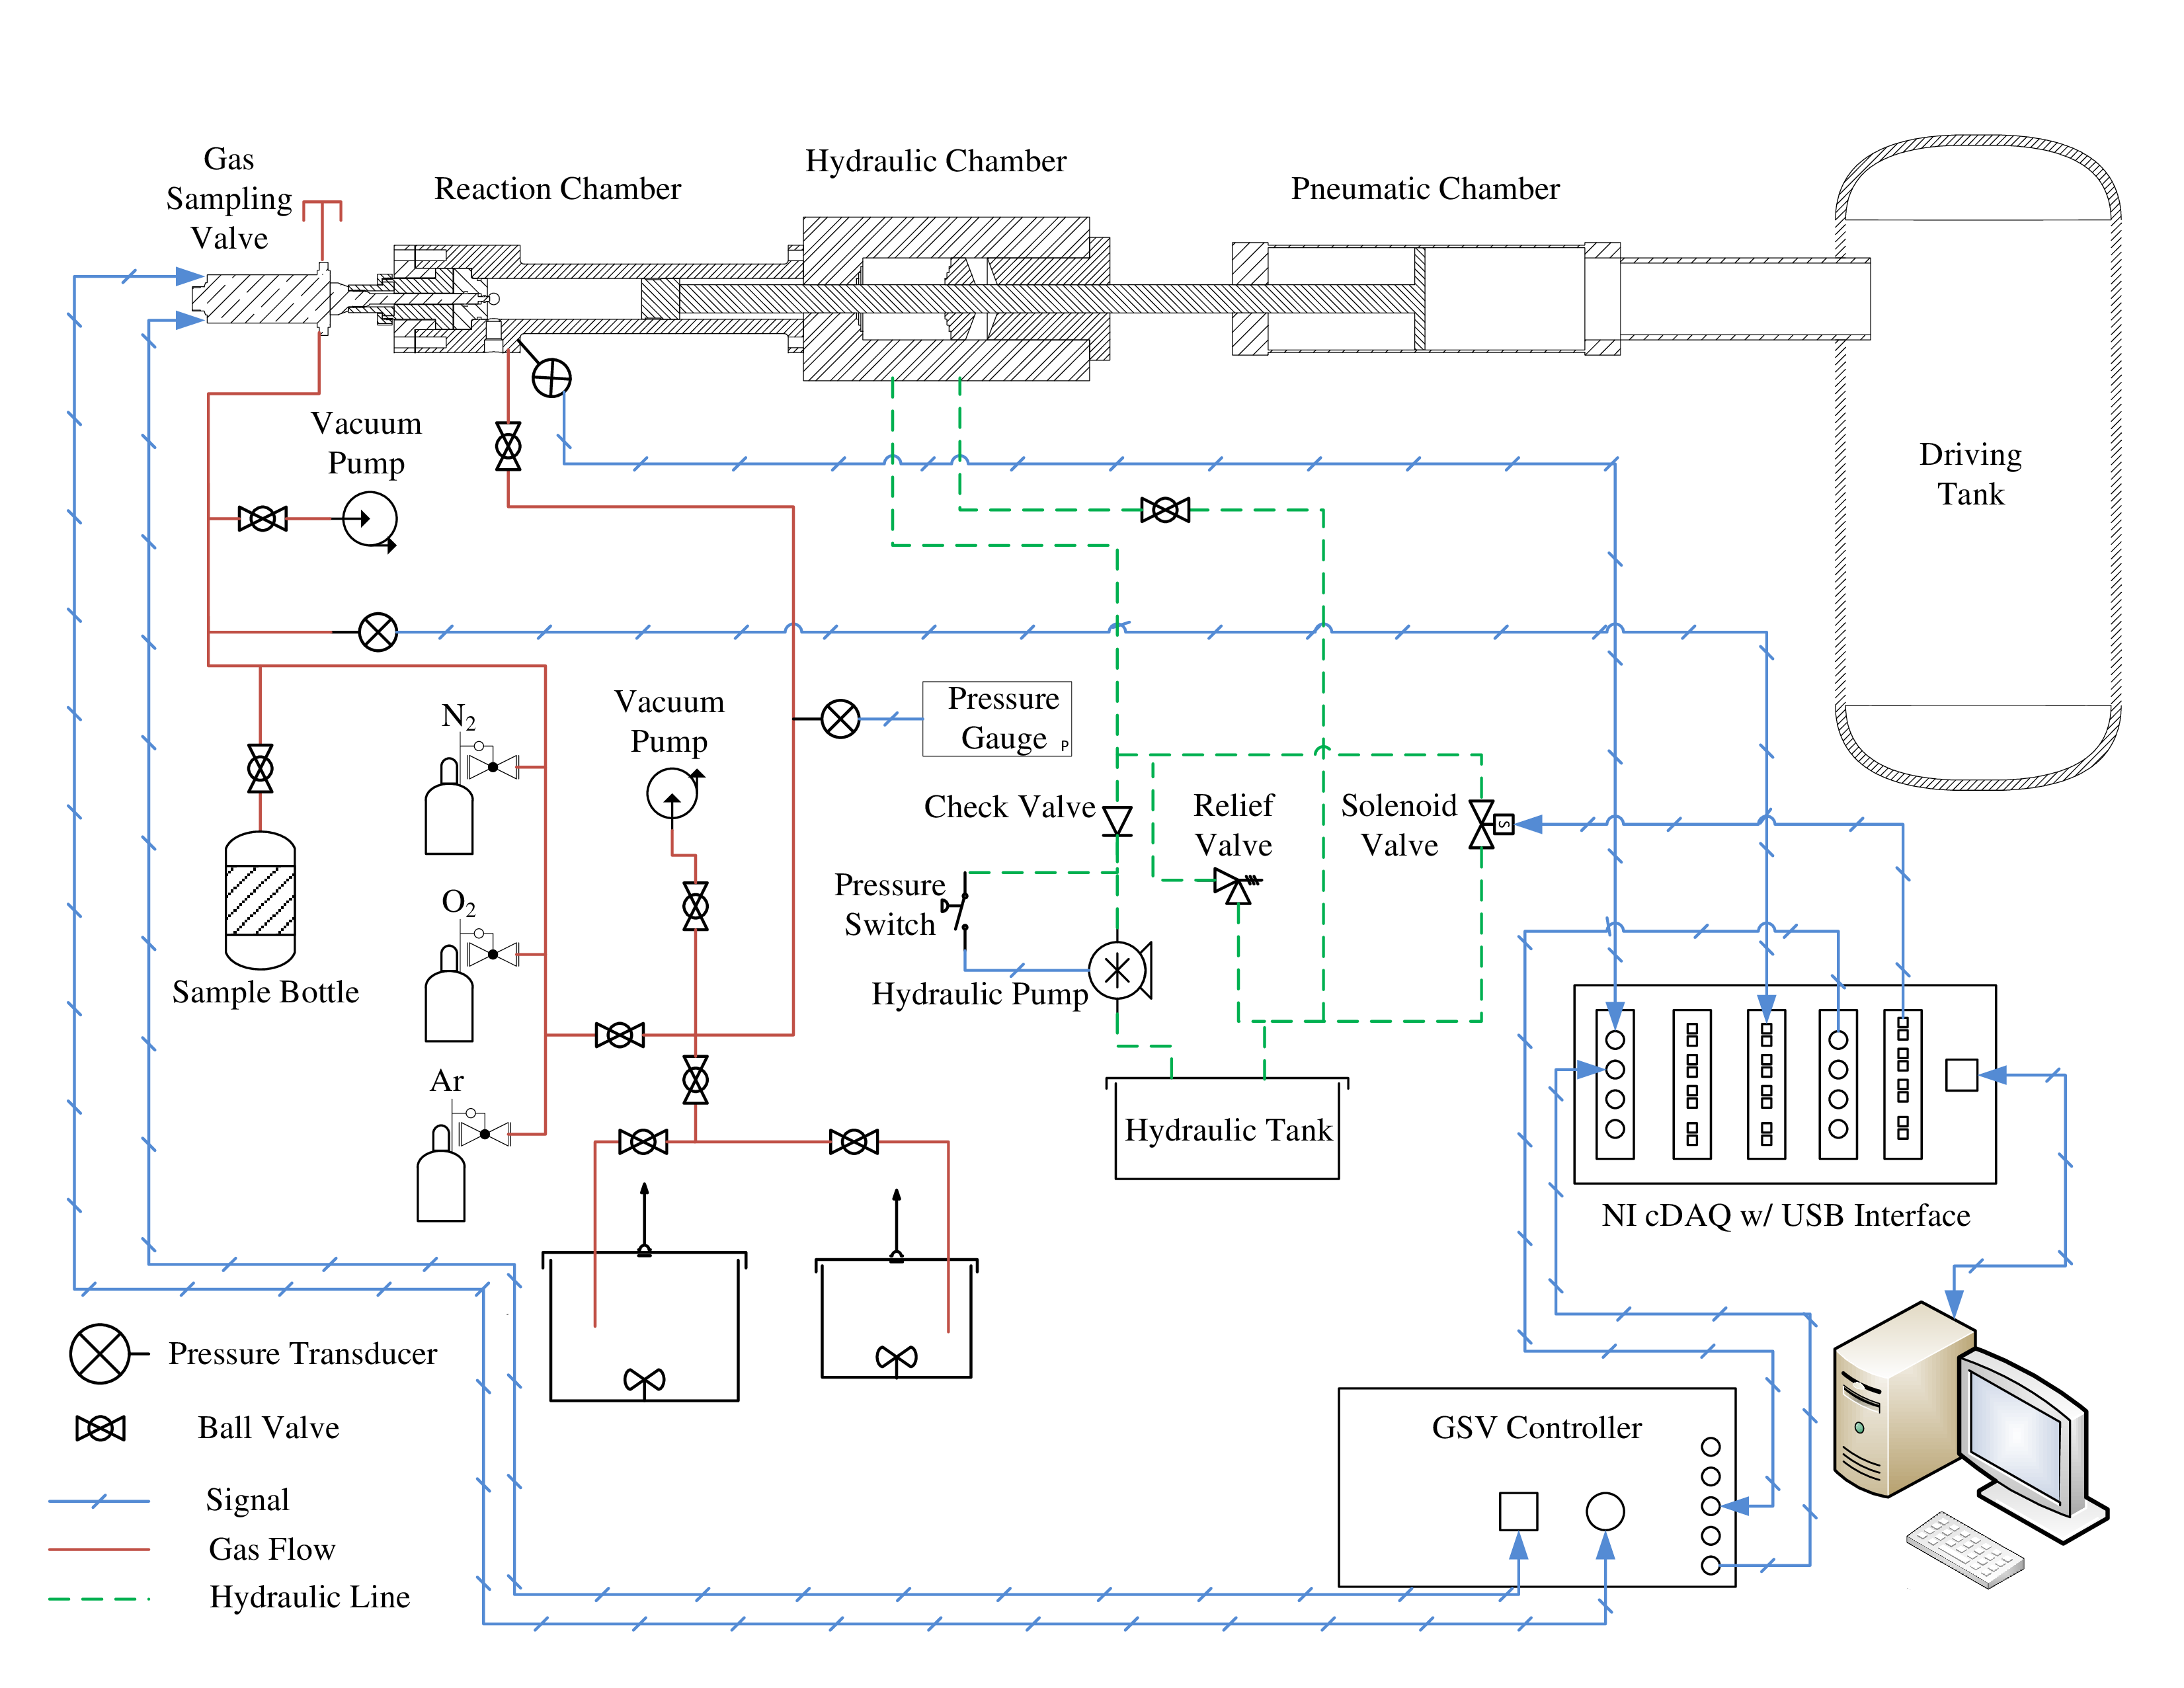
\includegraphics[width=\linewidth]{02-Experimental-Facilities/rcm-schematic}
\caption{Schematic of the RCM. Not to scale}
\label{fig:rcm-schematic}
\end{sidewaysfigure}
%\end{landscape}

\begin{figure}
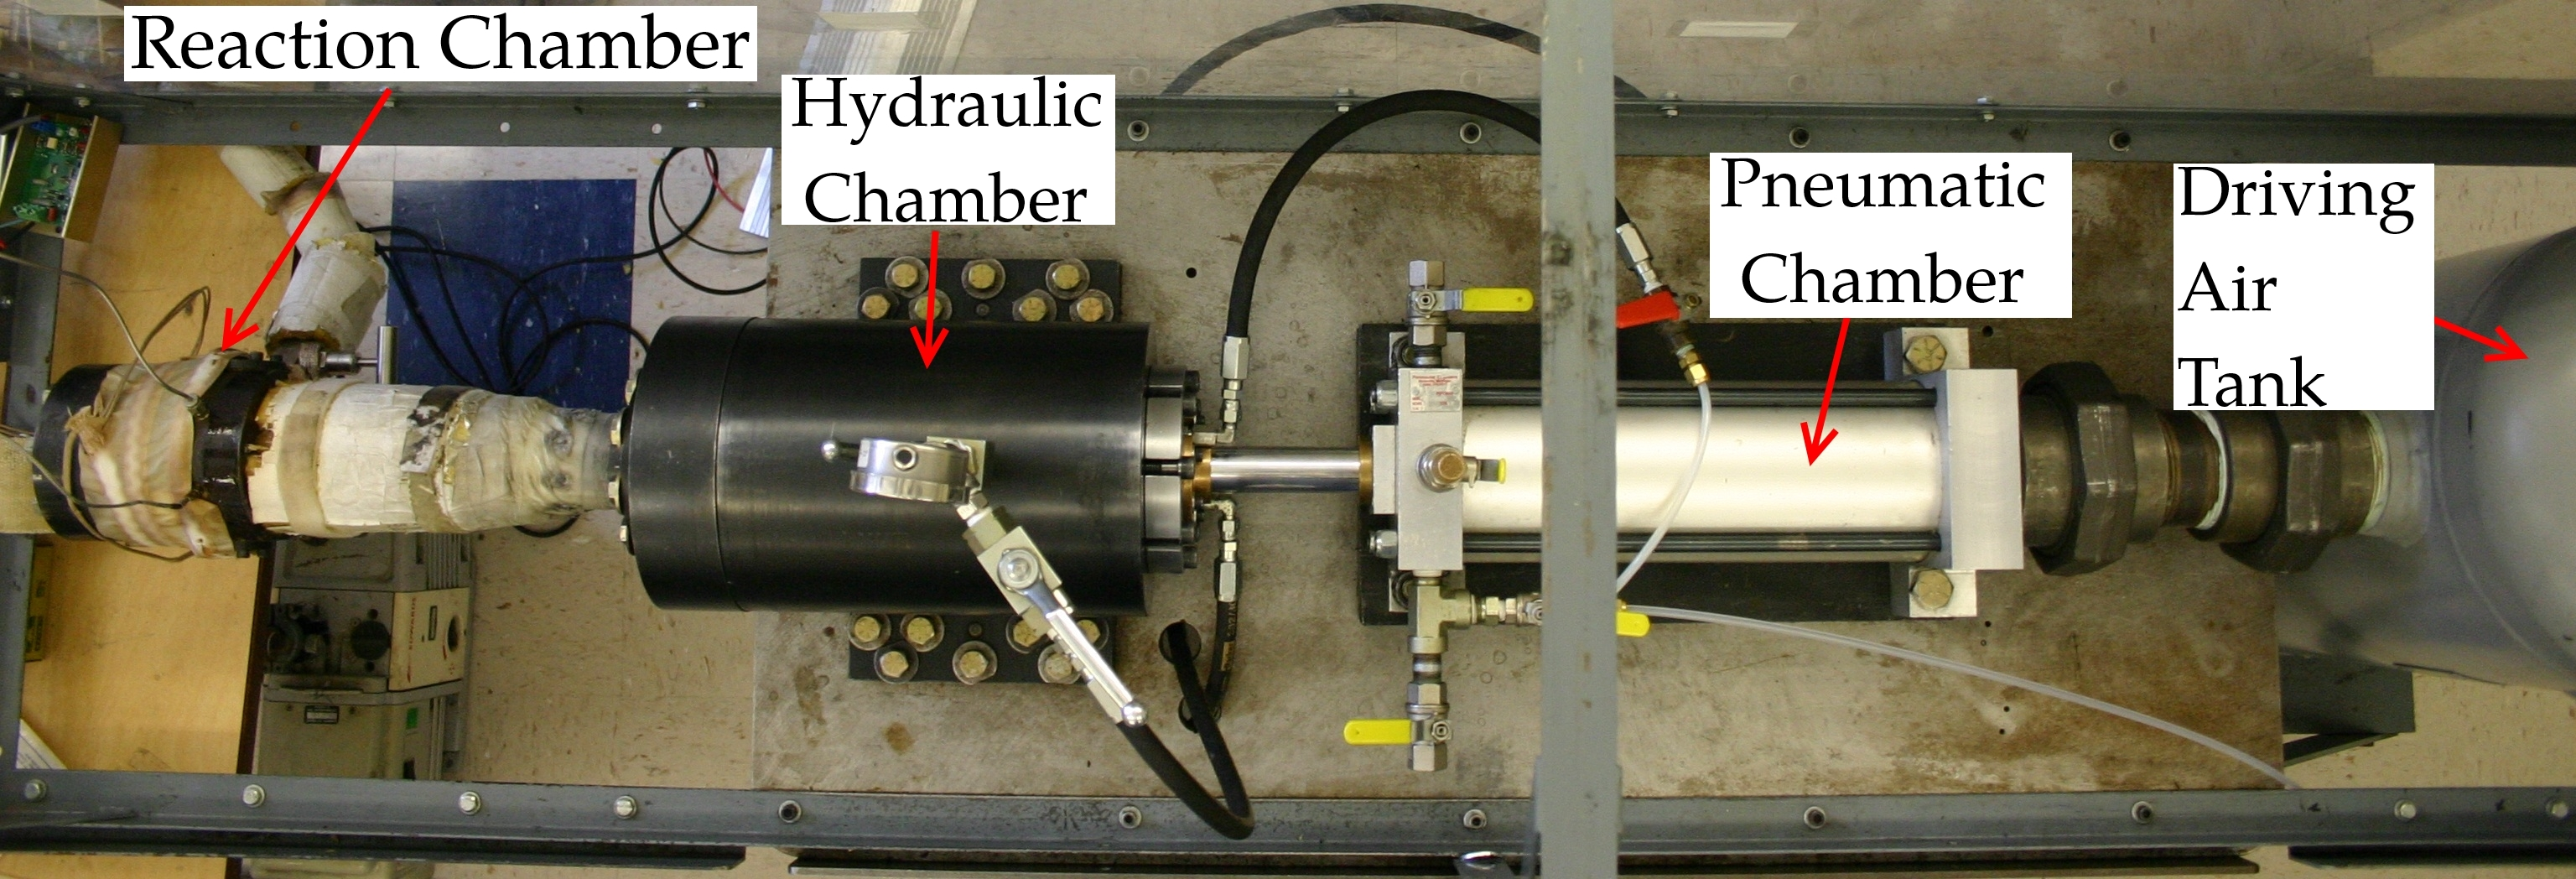
\includegraphics[width=5.7in]{02-Experimental-Facilities/rcm-photo}
\caption{Photograph of the RCM.}\label{fig:rcm-photo}
\end{figure}

At the start of an experimental run, with the piston in the
EOC position, the reaction chamber is vacuumed to less
than \SI{1}{\torr}. Next, the piston assembly is retracted by pressurizing
the front face of the piston in the pneumatic chamber.
For safety, and to prevent damage to the RCM, the driving tank should
be filled to limit the acceleration of the piston assembly during the
retraction.
The pressure on the front of the pneumatic piston pulls the
piston assembly rearward and seats the rear of the
hydraulic piston onto an O-ring in the rear of the
hydraulic chamber. The hydraulic chamber is filled with oil to
a pressure of approximately \SI{800}{psi}, providing a rearward force on the
front face of the hydraulic piston. Then, the air pressure is released from
the front of the pneumatic chamber and the driving tank is filled to
the desired driving pressure. The
force on the hydraulic piston opposes the force on the pneumatic piston
from the driving tank and the piston assembly remains at rest. Then, the
reaction chamber is filled with the required initial pressure of test
gas mixture from the mixing tank. Finally, compression is triggered by
releasing the hydraulic pressure through an electrically-operated solenoid
valve. The piston assembly is driven forward by the unbalanced force from
the pressure in the driving tank on the pneumatic piston. The gases
in the reaction chamber are brought to the compressed pressure ($P_C$) and
compressed temperature ($T_C$) conditions in approximately
\SIrange{30}{50}{\milli\second}.

The required driving pressure for a given EOC pressure can be estimated
from a force balance between the force on the pneumatic piston from the
driving tank and the force on the reactor piston from the test gases,
as shown in \cref{eq:driving-pressure}.
%
\begin{subequations}
\label{eq:piston-force}
\begin{align}
    P_{d,\text{min}} \cdot A_p &= P_{r,\text{EOC}} \cdot A_r \\
    P_{d,\text{min}} \cdot \frac{\pi d_p^2}{4} &= P_{r,\text{EOC}} \cdot \frac{\pi d_r^2}{4} \\
    P_{d,\text{min}} &= P_{r,\text{EOC}} \cdot \frac{d_r^2}{d_p^2} \label{eq:driving-pressure}
\end{align}
\end{subequations}

In \cref{eq:piston-force}, $P_{d,\text{min}}$ is the minimum
driving pressure, $A_p$ is the cross-sectional area of the pneumatic piston,
$P_{r,\text{EOC}}$ is the pressure in the reactor at the EOC (i.e. $P_C$),
$A_r$ is the cross-sectional area of the reactor piston, $d_p$ is the diameter
of the pneumatic piston, and $d_r$ is the diameter of the reactor piston.

The minimum driving pressure is such that the piston does not rebound at
the EOC due to pressure on the reactor piston. So that the driving
pressure can be much lower than the EOC pressure, the diameter ratio of
the reactor piston to the driver piston is \num{2/5}, allowing a factor of
\num{6.25} lower driving pressure than EOC pressure. The actual driving
pressure should exceed the minimum by some safety margin so that the
reactor remains at constant volume even if there is some pressure rise
due to heat release in the reaction chamber prior to the main ignition.

There is not a theoretical upper limit on the driving pressure. It is desired that the piston should
reach the EOC conditions in as short a time as possible to minimize heat
loss from the reactants to the reactor walls and minimize the time for
reactions to occur during the compression stroke. This implies that the
driving pressure should be made as high as possible so that the highest
piston velocity is achieved. However, higher piston velocities require
a higher deceleration at the EOC. In the present RCM, the deceleration
is provided by venting the hydraulic oil between steps on the hydraulic
piston and matched steps on the front of the hydraulic chamber. If the
piston is overdriven---that is, the driving pressure is too high---the
piston will not be sufficiently decelerated by the oil venting and will
impact the front of the hydraulic chamber at high velocity. This can damage
the RCM and cause the piston to rebound elastically. It also generates
substantial noise in the pressure trace and should be avoided.

Typical driving gas pressures are between \SI{50}{psi} for $P_C = \SI{15}{\bar}$ experiments
to  \SI{125}{psi} for $P_C = \SI{50}{\bar}$ experiments. These driving pressures represent a
good compromise between the minimum required for no rebound at EOC due
to pressure and no rebound at EOC due to elastic reaction. Nonetheless,
a small amount of piston rebound can be expected during/after the
main ignition event. This small rebound may have an effect on the computation of
ignition delay if it reduces the pressure rise rate during the ignition;
it is expected that this effect will be very small relative to the
typical random uncertainty in ignition delay experiments. Moreover,
the driving pressures required to balance the full pressure rise during
to ignition are more likely cause elastic rebound,
especially for high $P_C$ when the post-ignition pressure rise is greater.

The EOC conditions ($P_C$ and $T_C$) can be independently varied. This
is made possible by independent variation of the compression ratio,
initial pressure and initial temperature, and the specific heat ratio
of the test gases. The compression ratio can be
increased by adding spacers onto the rear of the hydraulic chamber,
increasing the stroke, and can be reduced by adding split shims onto
the rear of the reaction chamber, increasing the EOC clearance length.
Adjustment of the specific heat ratio of the gas can be accomplished
by substituting components (i.e. substituting Ar for N$_2$ results in
higher $P_C$ and $T_C$ if all other conditions are fixed). The initial
temperature is controlled by heaters, as described in the following
section.

\subsection{Test Gas Mixture Preparation}

Fuel/oxidizer pre-mixtures are prepared in two mixing tanks, one approximately
\SI{17}{\liter} and the other approximately \SI{15}{\liter} in volume. These large volumes allow many
runs to be conducted from one mixture preparation. The mixing tanks are connected
to the reaction chamber by flexible stainless steel manifold tubing. The tanks, reaction chamber,
and connecting manifold are wrapped in heating tape and insulation to control the initial
temperature of the mixture. Temperature controllers from Omega Engineering use thermocouples
placed on the lid of each mixing tank, approximately in the center of each mixing tank, embedded in
the wall of the reaction chamber, and near the inlet valve of the reaction chamber to control the
preheat temperature of the mixture. A static pressure transducer
measures the pressure in the manifold and mixing tanks. This transducer is used
during mixture preparation and to measure the initial pressure of a given experiment.
Two transducers are for various experiments in this work, as described below
in \cref{sec:unc-p0}.

Most of the fuels studied in this work are liquids at room temperature and
pressure and have relatively low vapor pressure. A similar procedure, outlined
below, was used for all of the butanol isomers, \textit{iso}-pentanol, and
methylcyclohexane; specific procedures are given in the chapter relevant to
each fuel. First, the mixing tanks are vacuumed to an ultimate pressure
less than \SI{5}{\torr}. The liquid fuel is massed in a syringe to a precision of
\SI{0.01}{\gram} prior to injection through a septum. Proportions of O$_2$, N$_2$, and
Ar are added manometrically at room temperature. The preheat temperature of
the RCM is set above the saturation point for each fuel to ensure complete
vaporization. The vapor pressure as a function of temperature is calculated
according to fits taken from \textcite{Yaws1999}. A magnetic stirrer mixes
the reactants. The temperature inside the mixing tank is allowed to
equilibrate for approximately \SI{1.5}{\hour}.

This approach to mixture preparation has been validated in several previous
studies by withdrawing gas samples from the mixing tank and analyzing the
contents by GC/MS \cite{Weber2011}, GC-FID \cite{Kumar2009}, and GC-TCD
\cite{Das2012}. These studies have verified the concentration of
\textit{n}-butanol, \textit{n}-decane, and water, respectively. In addition,
both the work by \textcite{Kumar2009} on \textit{n}-decane and the study of
\textcite{Weber2011} on \textit{n}-butanol confirmed that there was no fuel
decomposition over the course of a typical set of experiments. Furthermore,
within this study, each new mixture preparation is checked against previously
tested conditions to ensure reproducibility.

\subsection{Definition of Ignition Delay}
\label{sec:ig-delay-def}

The pressure in the reaction chamber during an experiment is monitored by a
Kistler 6125B piezoelectric dynamic pressure transducer. The charge signal from the
transducer is amplified and converted to a voltage by a Kistler 5010B charge amplifier.
The voltage is sent to a National Instruments cDAQ equipped with the NI-9215 module.
The signal is recorded by a LabView VirtualInstrument at \SI{50}{\kilo\hertz}.

\Cref{fig:ig-delay-def} shows a representative pressure trace from
these experiments with methylcyclohexane (MCH) at $P_C= \SI{50}{\bar}$, $T_C=\SI{761}{\kelvin}$,
and $\phi=\num{1.5}$ (See \cref{chap:mch}). Note that \cref{fig:ig-delay-def}
shows a case with two stages of ignition; not all of the fuels studied
had conditions that showed two-stage ignition. Nonetheless, the ignition
delay is consistently defined in all the work in this study. The
definitions of the EOC and the ignition delays are indicated on the figure.
The end of compression time is defined as the time when the pressure
reaches its maximum before first stage ignition occurs, or for cases
where there is no first stage ignition, the maximum pressure before
the overall ignition occurs. The first stage ignition delay is the time
from the end of compression until the first peak in the time derivative
of the pressure. The overall ignition delay is the time from the end of
compression until the largest peak in the time derivative of the pressure.

\begin{figure}
    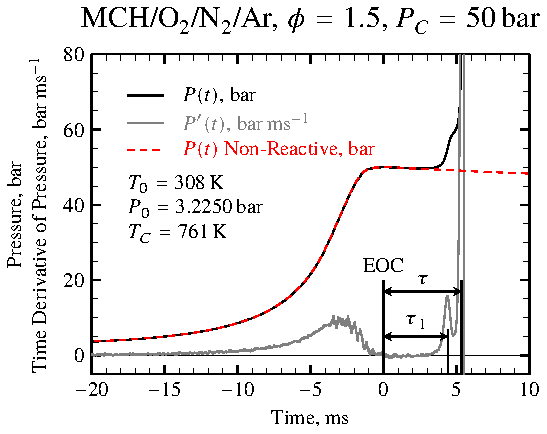
\includegraphics[width=12cm]{02-Experimental-Facilities/ign-delay-def}
    \caption{Representative pressure trace indicating the definition of
    the first stage and overall ignition delays and the corresponding
    non-reactive pressure trace. EOC stands for End of Compression.}
    \label{fig:ig-delay-def}
\end{figure}

Each unique $P_C$ and $T_C$ condition is repeated at least 5 times to
ensure repeatability of the experiments. The experiment closest to the
mean of the runs at a particular condition is chosen for analysis and
presentation. The standard deviation of all of the runs at a condition
is less than 10\% of the mean in all cases.

\subsection{Non-Reactive Experiments}

\Cref{fig:ig-delay-def} also shows a non-reactive pressure trace.
Due to heat loss from the test mixture to the cold reactor walls,
the pressure and temperature of the gas in the reaction chamber will
decrease after the end of compression. A non-reactive pressure trace
is measured that corresponds to each unique $P_C$ and $T_C$ condition
studied to quantify the effect of the heat loss on the ignition process
and to verify that no heat release has occurred during the compression
stroke. The non-reactive pressure trace is acquired by replacing the
oxygen in the oxidizer with nitrogen, so that the specific heat ratio
of the initial mixture is maintained, but the heat release due to
exothermic oxidation reactions is eliminated. Maintaining a similar
specific heat ratio ensures that the non-reactive experiment faithfully
reproduces the conditions of the reactive experiment. A representative
non-reactive pressure trace is shown in \cref{fig:ig-delay-def}
corresponding to the experimental conditions in the figure.

\subsection{Reaction Chamber Homogeneity}

An RCM to be used for studies of homogeneous chemistry---as in this study---%
must ensure that homogeneous conditions exist inside the reaction
chamber for the duration of the experiment. Due to the high piston
velocities required to minimize heat loss and reaction during the
compression stroke, complex fluid mechanical effects can strongly
affect the state of the reactants at the EOC. The most important of these
effects is caused by the motion of the piston itself, where the piston
pushes the wall boundary layer into a roll-up vortex \cite{Lee1998}.
This cold vortex mixes with the hotter gases near the center of
the reaction chamber and causes large spatial inhomogeneities of
temperature and species.

To facilitate spatially homogeneous conditions in the reactor
and reduce the effect of the roll-up vortex, it is necessary to trap
the boundary layer. This is accomplished on the present RCM by a
crevice machined into the crown of the piston, shown in cross-section
in \cref{fig:rcm-piston}. The boundary layer enters the crevice through
the converging section as the piston moves forward and is trapped
within the crevice. The dimensions of the crevice were optimized
by \textcite{Mittal2006a} through CFD simulations. Subsequently,
\textcite{Mittal2006b} experimentally showed that the optimized crevice
design provides homogeneous conditions in the reaction chamber up to
approximately \SI{150}{\milli\second} after the EOC. By using PLIF
measurements of acetone-seeded mixtures, \textcite{Mittal2006b}
showed that there was a core region of gases near the center of the
reactor whose temperature remained spatially homogeneous.

\begin{figure}[!ht]
    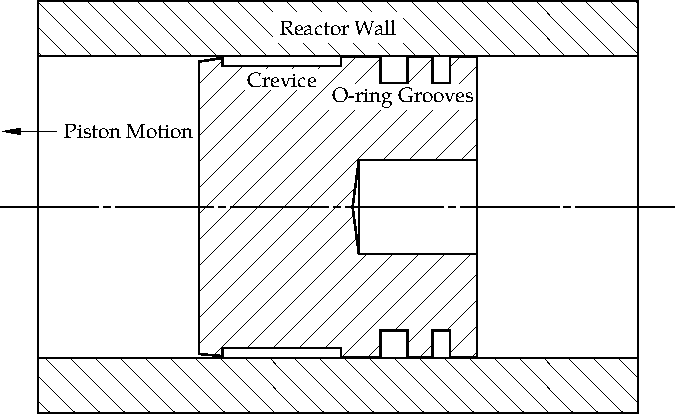
\includegraphics[width=12cm]{02-Experimental-Facilities/rcm-piston}
    \caption{Creviced piston installed in the present RCM.}
    \label{fig:rcm-piston}
\end{figure}

\subsection{Determination of Reactant Temperature}

In general, it is rather difficult to directly measure the temperature
of the gases in the reaction chamber during and after compression.
Intrusive methods such as thermocouples may introduce inhomogeneities into
the reaction chamber and non-intrusive optical techniques are difficult to set up
and require extensive calibration at the pressures of interest in RCM
studies. Thus, the temperature is determined indirectly by applying an
assumption called the ``adiabatic core hypothesis'' to the reaction chamber
\cite{Mittal2007, Lee1998}.

If all of the gases in the reaction chamber were compressed isentropically,
the temperature at the end of compression could be found by the
following relations:
%
\begin{subequations}
\label{eq:tic}
\begin{align}
\ln\left(\text{CR}\right) = \int_{T_0}^{T_{ic}} \! \frac{1}{T\left(\gamma-1\right)} \, \mathrm{d} T \\
\ln\left(\frac{P_{ic}}{P_0}\right) = \int_{T_0}^{T_{ic}} \! \frac{\gamma}{T\left(\gamma-1\right)} \, \mathrm{d} T
\end{align}
\end{subequations}
%
where CR is the volumetric compression ratio, $T_0$ is the initial temperature,
$T_{ic}$ is the temperature at the end of isentropic compression, $\gamma$ is the
temperature-dependent ratio of specific heats, $P_{ic}$ is the pressure at the
end of isentropic compression, and $P_0$ is the initial pressure.

However, experiments show that the measured pressure in the reaction chamber
does not reach the value of $P_{ic}$ calculated by using the geometric
compression ratio. The difference is due to finite heat loss from the
reactants to the reactor walls and the crevice volume during the
compression. Under the adiabatic core hypothesis, it is assumed that
the heat loss from the reactants only occurs in a thin boundary layer
near the wall, and the central core region is unaffected by heat loss
(i.e. the core is adiabatic) \cite{Desgroux1995}. Thus, the heat
loss is modeled as an effective reduction in the compression ratio, and
the temperature during the compression stroke can be calculated by:
%
\begin{align}
\ln\left(\frac{P_{C}}{P_0}\right) = \int_{T_0}^{T_{C}} \! \frac{\gamma}{T\left(\gamma-1\right)} \, \mathrm{d} T
\label{eq:tc}
\end{align}
%
where $P_C$ is the measured pressure at the end of compression, $T_C$
is the temperature at the end of compression, and the other variables
are the same as in \cref{eq:tic}.

After the end of compression, the pressure in the reaction chamber
decreases, as can be seen in \cref{fig:ig-delay-def}. This pressure
decrease is caused by heat loss from the reactants in the constant volume reaction
chamber and is accompanied by a decrease in the temperature of the
reactants. To model the thermodynamic state after the end of compression,
the adiabatic core hypothesis is applied and the heat loss is
assumed to occur only in a thin boundary layer near the reactor walls.
Thus, the core region is modeled as adiabatic, and the heat loss
from the boundary layer is be modeled as an isentropic volume
expansion.

In general, the specific heat ratio used in \cref{eq:tic,eq:tc} is an
unknown function of temperature and composition, so \cref{eq:tc}
cannot be integrated directly to find $T_C$. If the specific heats are
parameterized with a linear fit and the composition is assumed to be
fixed, it is possible to integrate \cref{eq:tc} directly, but this
process is quite tedious; nonetheless, it will be applied in
\cref{sec:uncertainty} to determine the uncertainty of $T_C$. In
general, the simplest method of calculating $T_C$ is to use software
to numerically integrate \cref{eq:tc}.

In this work, the CHEMKIN-Pro \cite{Chemkin2012} software is used to
perform the numerical integration and calculation of $T_C$. The
CHEMKIN-Pro software provides the facility for a user-specified
volume as a function of time to be applied to a homogeneous,
adiabatic reactor. Since the adiabatic core of the reaction chamber
is modeled as undergoing an isentropic volumetric compression followed
by an isentropic volumetric expansion, the user-specified volume
functionality is used to compute the RCM reactor state as a function
of time. A volume trace for simulation is computed from the measured
pressure trace using the isentropic relation:
%
\begin{align}
\frac{V_2}{V_1} = \left[\frac{P_1}{P_2}\right]^{\frac{1}{\gamma}}
\label{eq:volume-trace}
\end{align}
%
where $V_1$ and $V_2$ are the volumes at consecutive time points,
$P_1$ and $P_2$ are the pressures at consecutive time points, and
$\gamma$ is the temperature dependent specific heat. This equation
is applied during and after the compression stroke to calculate
the volume trace. Since the non-reactive experiment requires slightly
different initial pressure (on the order of 5 torr) to reach the same
compressed pressure as the reactive experiment---due to the slightly
different specific heat ratio in the non-reactive experiment as compared
to the reactive experiment---the reactive pressure trace is used to
compute the volume trace until EOC; after EOC, the corresponding
non-reactive pressure trace is used. In \cref{eq:volume-trace} it is assumed that
changes in composition of the reactants are negligible during the
compression stroke, which is confirmed by comparing simulations with and
without reaction steps in the chemical kinetic model. The EOC conditions
are the same in both cases. The initial volume is arbitrarily taken
to be equal to 1.

For use in \cref{eq:volume-trace}, the temperature-dependent specific
heat ratio $\gamma$ is tabulated for each time point. Thus, the
temperature at each time point must also be computed by using the
isentropic relation for temperature:
%
\begin{align}
\frac{T_2}{T_1} = \left[\frac{P_2}{P_1}\right]^{\frac{\gamma-1}{\gamma}}
\label{eq:isen-temp}
\end{align}
%
where $T_2$ and $T_1$ are the temperatures at consecutive time points.
Since $T_2$ depends on the value of $\gamma$, which in turn depends
on $T_2$, \cref{eq:isen-temp} is iterated until the temperature
changes by less than one tenth of one percent on consecutive iterations.
Once again, it is assumed that changes in composition have a negligible
influence on the ratio of specific heats.
The temperature calculated by \cref{eq:isen-temp} is typically within
1K of the temperature calculated by CHEMKIN-Pro.

\subsection[Uncertainty of Compressed Temperature and Ignition Delay]%
{Uncertainty of Compressed Temperature\\ and Ignition Delay}
\label{sec:uncertainty}

The uncertainty of the compressed temperature is an important parameter
to report. Since $T_C$ is not measured, we must perform an uncertainty
propagation analysis on the equation used to calculate $T_C$,
\cref{eq:tc}. First, we simplify the term involving $\gamma$ in
\cref{eq:tc}. By definition, $\gamma$ is the ratio of the specific heat
at constant pressure to that at constant volume
%
\begin{align}
\gamma \equiv \frac{C_p}{C_v} = \frac{C_p/R}{C_v/R} = \frac{\hat{C}_p}{\hat{C}_v}
\end{align}
%
where $C_p$ and $C_v$ are the specific heats in molar units at constant
pressure and volume, respectively, and $R$ is the universal gas constant,
used to produce non-dimensional specific heats, indicated by a hat. The
difference between the non-dimensional specific heats is one,
$\hat{C}_v = \hat{C}_p - 1$. Then, it follows that
%
\begin{align}
\label{eq:simplify-gamma}
\frac{\gamma}{\gamma - 1} = \frac{\frac{\hat{C}_p}{\hat{C}_v}}{\frac{\hat{C}_p}{\hat{C}_v} - 1}
= \frac{\frac{\hat{C}_p}{\hat{C}_p - 1}}{\frac{\hat{C}_p}{\hat{C}_p - 1} - 1}
= \frac{\frac{\hat{C}_p}{\hat{C}_p - 1}}{\frac{1}{\hat{C}_p - 1}}
= \hat{C}_p
\end{align}

In \cref{eq:tc}, the total specific heat ratio for the mixture
should be used; thus, the simplification as shown in \cref{eq:simplify-gamma}
requires that the specific heat $\hat{C}_p$ also be the total specific
heat. In the following, we assume that there is negligible
change of the total specific heat due to changes in reactant
mole fractions, as for \cref{eq:volume-trace,eq:isen-temp}.
The total specific heat is simply the sum of the product of
the species mole fractions and their specific heats
%
\begin{subequations}
\label{eq:cp}
\begin{align}
C_{p\text{,total}} &= \sum_i X_i C_{p,i} \\
\hat{C}_{p\text{,total}} &= \frac{\sum_i X_i C_{p,i}}{R}
\end{align}
\end{subequations}
%
where $i$ indicates the species and $X_i$ is the species mole fraction.
In the NASA polynomial formulation used by CHEMKIN, the non-dimensional specific
heat at constant pressure as a function of temperature is represented by a
fourth-order polynomial fit
%
\begin{align}
\label{eq:cp-nasa}
\hat{C}_{p,i} = c_{1,i} + c_{2,i} T + c_{3,i} T^2 + c_{4,i} T^3 + c_{5,i} T^4
\end{align}
%
In general, this means that the specific heat can be non-linear. However,
since the mixtures prepared in this study are composed primarily of
O$_2$, N$_2$ and Ar (i.e. no more than 7\% of any mixture is the
fuel), and since the specific heats of O$_2$, N$_2$ and Ar are only weakly
temperature dependent over the range of temperatures experienced during
compression, for the purposes of this uncertainty analysis, we will
approximate the total specific heat as a linear function of temperature:
%
\begin{equation}
\label{eq:cp-total}
\begin{split}
\hat{C}_{p\text{,total}} &= \sum_i X_i \hat{C}_{p,i} \\
&= \sum_i X_i \left( \sum_{j=1}^5 c_{j,i} T^{j-1} \right) \\
&\approx a + b T
\end{split}
\end{equation}
%
$a$ and $b$ are found by fitting the total non-dimensional specific heat
over the temperature range from \SIrange{300}{1100}{\kelvin}, as
discussed below in \cref{sec:unc-cp}.

With this approximation of the specific heat, we can integrate \cref{eq:tc}
to find the compressed temperature
%
\begin{subequations}
\begin{align}
\ln{\frac{P_C}{P_0}}
&= \int_{T_0}^{T_{C}} \! \frac{\gamma}{T\left(\gamma-1\right)} \, \mathrm{d} T \\
&= \int_{T_0}^{T_{C}} \! \frac{\hat{C}_p}{T} \, \mathrm{d} T \\
&= \int_{T_0}^{T_{C}} \! \frac{a + b T}{T} \, \mathrm{d} T\\
&= \Big[a \ln{T} + b T \Big]_{T_0}^{T_C}
\end{align}
\begin{equation}
\ln{\frac{P_C}{P_0}} + \left(a \ln{T_0} + b T_0\right) = a \ln{T_C} + b T_C \label{eq:integrate-tc}
\end{equation}
\end{subequations}

\Cref{eq:integrate-tc} can be solved explicitly for $T_C$ by using
Lambert's $W$ function \cite{Corless1996}, but this function is somewhat
complex. Instead, \cref{eq:integrate-tc} is simplified by performing a
Taylor expansion of the right hand side and solving for $T_C$:
%
\begin{gather}
a \ln{T_C} + b T_C \approx a \ln{T_e} + bT_e + \left(\frac{a}{T_e} + b\right)\left(T_C - T_e\right) \\
T_C = \frac{\ln{\frac{P_C}{P_0}} + a \ln{\frac{T_0}{T_e}} + b\left(T_0 - T_e\right)}{\frac{a}{T_e}+b} + T_e \label{eq:explicit-tc}
\end{gather}
%
where $T_e$ is the temperature about which the Taylor expansion is performed.

With an explicit function for $T_C$, we can estimate the uncertainty in
$T_C$ by the root square sum of the uncertainty in the parameters in
\cref{eq:explicit-tc} multiplied by the partial derivative of
\cref{eq:explicit-tc} with respect to each of the parameters
\cite{Taylor1982}. The parameters are $P_C$, $P_0$, $T_0$, $a$, and $b$
and are assumed to be independent.
%
\begin{align}
\label{eq:tc-unc}
U_{T_C} = \sqrt{\left(\frac{\partial T_C}{\partial P_C} U_{P_C}\right)^2 + \left(\frac{\partial T_C}{\partial P_0} U_{P_0}\right)^2 +
                \left(\frac{\partial T_C}{\partial T_0} U_{T_0}\right)^2 + \left(\frac{\partial T_C}{\partial a} U_{a}\right)^2 +
                \left(\frac{\partial T_C}{\partial b} U_{b}\right)^2}
\end{align}

The uncertainties of the parameters, $U_j$ in \cref{eq:tc-unc}, are in
general found by their own root square sum procedure
%
\begin{align}
{U_j}^2 = {B_j}^2 + {R_j}^2
\end{align}
%
where the subscript $j$ represents one of the parameters in \cref{eq:explicit-tc}.
The total uncertainty of a particular parameter is composed of
two parts, the systematic or bias uncertainty ($B_j$) and the
precision or random uncertainty ($R_j$). In general, the bias
uncertainty is contained in the measurement equipment and can
be reduced, e.g. by using different equipment; the random uncertainty
is inherent in any measured process and cannot be reduced by
experimental techniques. The bias and precision uncertainties
for each parameter will be discussed in the following sections.

The partial derivatives of \cref{eq:explicit-tc} with respect to
each of the parameters are given in \cref{eq:partial-derivs}:
%
\begin{subequations}
\label{eq:partial-derivs}
\begin{gather}
\frac{\partial T_C}{\partial P_C} = \frac{T_e}{P_C\left(a + T_e b\right)} \displaybreak[0]\\[1em]
\frac{\partial T_C}{\partial P_0} = \frac{-T_e}{P_0\left(a + T_e b\right)}\displaybreak[0]\\[1em]
\frac{\partial T_C}{\partial T_0} = \frac{T_e\left(a + T_0 b\right)}{T_0\left(a + T_e b\right)}\displaybreak[0]\\[1em]
\frac{\partial T_C}{\partial a} = \frac{T_e \left[b \left(T_e \ln{\frac{T_0}{T_e}} + T_e - T_0 \right) - \ln{\frac{P_C}{P_0}} \right]}{\left(a + T_e b \right)^2} \displaybreak[0]\\[1em]
\frac{\partial T_C}{\partial b} = -\frac{T_e \left[a \left(T_e \ln{\frac{T_0}{T_e}} + T_e - T_0 \right) + T_e \ln{\frac{P_C}{P_0}}\right]}{\left(a + T_e b \right)^2}
\end{gather}
\end{subequations}

\subsubsection{Uncertainty in Initial Temperature}

The bias uncertainty in the initial temperature is due to the standard
limits of error of the K-type thermocouple used to measure the
initial temperature. According to the Omega Engineering
specifications, this is ``the greater
of $\SI{2.2}{\degreeCelsius}$ or 0.75\%''. The largest initial temperature
used in this work, \SI{413}{\kelvin}, leads to an uncertainty of
$\pm \SI{3}{\kelvin}$; thus, $B_{T_O}=\SI{3}{\kelvin}$. Bias uncertainty
due to the A/D converter in the process meter is negligible compared
to this uncertainty.
The precision uncertainty is due to the limit of precision of
the display on the Omega Engineering CNi3254 process meter used
to control the process temperature. This is $\pm\SI{0.05}{\kelvin}$.
The total uncertainty of the initial temperature is
%
\begin{align}
U_{T_0} = \sqrt{\left(B_{T_0}\right)^2 + \left(R_{T_0}\right)^2} = \sqrt{\left(\SI{3}{K}\right)^2 + \left(\SI{0.05}{K}\right)^2} = \SI{3}{\kelvin}
\end{align}

\subsubsection{Uncertainty in Initial Pressure}
\label{sec:unc-p0}

The bias uncertainty in the initial pressure is due to the
standard error in the pressure transducer used to measure
the initial pressure. Two different pressure transducers have
been used in this study; the first, an Omega Engineering PX-303
(range: \SIrange{0}{50}{psia}), has a full scale uncertainty of 1.25\%, or
$\pm \SI{0.625}{psi} \ (\SI{4309.2}{\pascal})$. The second transducer is an
Omega Engineering MMA100V10T2D0T4A6 type (range: \SIrange{0}{5200}{Torr}) and was
purchased because preliminary results of this uncertainty analysis
indicated that the largest contributor to the uncertainty of $T_C$ was
the initial pressure measurement. The full scale uncertainty of the MMA
type transducers is 0.05\%, resulting in an uncertainty of
$\pm \SI{2.6}{\torr} \ (\SI{346.6}{\pascal})$, an order of magnitude lower than
the PX-303 while also providing more than double the operating range. Total
uncertainties using the appropriate pressure transducer are reported in
each experimental section of this work; both transducers will be analyzed
in this section. Bias uncertainty due to the signal acquisition equipment
is negligible compared to the standard error in the pressure transducers.

The precision uncertainty is due to the limit of precision of the display
on the Omega Engineering DP41-B process meter used to monitor the initial
pressure. This is $\pm\SI{0.005}{\torr} \ (\SI{0.666}{\pascal})$. The total
uncertainty of the initial pressure is
%
\begin{subequations}
\begin{align}
U_{P_0} = \sqrt{\left(B_{P_0}\right)^2 + \left(R_{P_0}\right)^2} = \sqrt{\left(\SI{4309.2}{\pascal}\right)^2 + \left(\SI{0.666}{\pascal}\right)^2} = \SI{4309.2}{\pascal} \\
U_{P_0} = \sqrt{\left(B_{P_0}\right)^2 + \left(R_{P_0}\right)^2} = \sqrt{\left(\SI{346.6}{\pascal}\right)^2 + \left(\SI{0.666}{\pascal}\right)^2} = \SI{346.6}{\pascal}
\end{align}
\end{subequations}

\subsubsection{Uncertainty in Compressed Pressure}

The bias uncertainty in the compressed pressure is due to the standard
error in the piezoelectric pressure transducer. According to the
manufacturer's calibration, the deviation of the full scale output from
linearity is less then 0.1\% over the pressure range \SIrange{0}{50}{\bar},
indicating that $B_{P_C}=\SI{0.05}{\bar}=\SI{5000}{\pascal}$.
The uncertainties in the signal acquisition equipment are negligible
compared to this uncertainty. The precision uncertainty is due to the limit
of precision of the output of the pressure, and is \SI{5E-7}{\bar}. This
is negligible compared to the bias uncertainty, so the total uncertainty
of the compressed pressure is
%
\begin{equation}
U_{P_C} = B_{P_C} = \SI{0.05}{\bar} = \SI{5000}{\pascal}
\end{equation}

\subsubsection{Uncertainty in the Specific Heat}
\label{sec:unc-cp}

The uncertainty in the specific heat comes from two sources. First is the
uncertainty in the mixture composition and second is the uncertainty in
the linear fit to the total specific heat. The uncertainty in the mixture
composition can be estimated by the same method as is used for $T_C$. The
specific heat is given by \cref{eq:cp}, so we can take partial derivatives
of that equation with respect to the mole fractions of the species to find
the total uncertainty
%
\begin{equation}
\label{eq:cp-uncertainty}
\begin{split}
\left(U_{\hat{C}_{p\text{,total}}}\right)^2 &= \left(\frac{\partial \hat{C}_p}{\partial X_1} U_{X_1}\right)^2 + \ldots + \left(\frac{\partial \hat{C}_p}{\partial X_n} U_{X_n}\right)^2 \\
&= \left(\hat{C}_{p,1} U_{X_1}\right)^2 + \ldots + \left(\hat{C}_{p,n} U_{X_n}\right)^2
\end{split}
\end{equation}
%
where $n$ is the total number of species. In \cref{eq:cp-uncertainty},
it is assumed that the uncertainty in the specific heats of each species
is negligible. This is considered an acceptable assumption for stable species
such as the fuel molecules, oxygen, nitrogen, and argon. Experience with
several kinetic mechanisms has shown that the typical variation in individual
$\hat{C}_p$ fits causes approximately \SI{1}{\kelvin} changes in $T_C$.

The uncertainty of the mole fraction of the species is estimated differently
depending on how the species was introduced to the mixing tank. For liquid fuel
species, experiments with GC/MS have shown that there is approximately 5\%
variation in mole fraction from the expected value \cite{Weber2011}; this value is adopted for
the total uncertainty of all liquid fuels. The mole fraction of the gaseous species
is determined by their partial pressures when filling; the mole fraction is
related to the pressure by Dalton's Law of Partial Pressure
\cite{Dalton1801,Gillespie1930}
%
\begin{equation}
X_i = \frac{P_i}{P}
\end{equation}
%
where $P_i$ is the partial pressure of a species and $P$ is the total pressure.
It follows that
%
\begin{equation}
\begin{split}
\left(U_{X_i}\right)^2 &= \left(\frac{\partial X_i}{\partial P_i} U_{P_i}\right)^2 + \left(\frac{\partial X_i}{\partial P} U_P\right)^2 \\
&= \left(\frac{U_{P_i}}{P}\right)^2 + \left(\frac{{-P_i}}{P^2} U_P\right)^2
\end{split}
\end{equation}
%
The uncertainties of the pressures $P_i$ and $P$ are equal and can be estimated by
the same procedure as in \cref{sec:unc-p0} since the same pressure transducer
is used to measure the pressure. The total pressure $P$ will be different for
each species as it is filled. The order followed in these experiments is
liquid fuel injection, followed by oxygen, then nitrogen, then argon when
applicable. It is assumed that the uncertainty in each partial pressure
is independent of all the others for simplicity.

A line is fit through the end points of the total specific heat curve
via simultaneous solution of the equations
%
\begin{equation}
\label{eq:cp-line}
\begin{split}
\hat{C}_{p,2} = b T_2 + a \\
\hat{C}_{p,1} = b T_1 + a
\end{split}
\end{equation}
%
where $\hat{C}_{p,1}$ and $\hat{C}_{p,2}$ are the total specific heats
at $T_1$ and $T_2$ respectively; in this analysis, the temperatures are
\SI{300}{\kelvin} and \SI{1100}{\kelvin}. Solving \cref{eq:cp-line} for
$b$ and $a$ gives:
%
\begin{equation}
\begin{split}
b &= \frac{\hat{C}_{p,2} - \hat{C}_{p,1}}{T_2 - T_1} \\[0.5em]
a &= \frac{f_2 \hat{C}_{p,2} - f_1 \hat{C}_{p,1}}{f_2-f_1}
\end{split}
\end{equation}
%
where $f_1$ and $f_2$ are chosen so that $b$ is eliminated in
\cref{eq:cp-line}.

Uncertainty in the slope and $y$-intercept can be found by
%
\begin{equation}
\begin{split}
\left(U_{b}\right)^2 = \left(\frac{\partial b}{\partial \hat{C}_{p,1}}U_{C_{p,1}}\right)^2 + \left(\frac{\partial b}{\partial \hat{C}_{p,2}}U_{C_{p,2}}\right)^2 \\[0.5em]
\left(U_{a}\right)^2 = \left(\frac{\partial a}{\partial \hat{C}_{p,1}}U_{C_{p,1}}\right)^2 + \left(\frac{\partial a}{\partial \hat{C}_{p,2}}U_{C_{p,2}}\right)^2
\end{split}
\end{equation}
%
where the partial derivatives are
%
\begin{align}
\frac{\partial b}{\partial \hat{C}_{p,1}} &= \frac{-1}{T_2 - T_1} & \frac{\partial b}{\partial \hat{C}_{p,2}} &= \frac{1}{T_2 - T_1} \\
\frac{\partial a}{\partial \hat{C}_{p,1}} &= \frac{-f_1}{f_2 - f_1} & \frac{\partial a}{\partial \hat{C}_{p,2}} &= \frac{f_2}{f_2 - f_1}
\end{align}
%
and the uncertainties of the specific heats $U_{C_{p,1}}$ and $U_{C_{p,2}}$
are calculated as described earlier.

\subsection{Uncertainty in Compressed Temperature}

The following analysis is considered for a representative mixture of
\SI{3.38}{\mole\percent} \tBuOH{}, \SI{20.30}{\mol\percent} O$_2$,
\SI{76.32}{\mole\percent} N$_2$, i.e. a $\phi=1.0$ mixture of \tBuOH{}
and air. A typical total pressure after filling is approximately
\SI{1520}{\torr} ($=\SI{202650}{\pascal}$), with approximately
\SI{42000}{\pascal} of O$_2$ and \SI{160650}{\pascal} of N$_2$. Thus,
the uncertainty in the mole fractions of the components are:
%
\begin{gather*}
\left(U_F\right)^2 = \left(0.0338 \cdot 0.05\right)^2 = \num{2.8561E-6} \\
\left(U_{O_2}\right)^2 = \left(\frac{\SI{4309.2}{\pascal}}{\SI{42000}{\pascal}}\right)^2 + \left(\frac{-\SI{4309.2}{\pascal}}{\SI{42000}{\pascal}}\right)^2 = \num{2.1054E-2} \\
\left(U_{O_2}\right)^2 = \left(\frac{\SI{ 346.6}{\pascal}}{\SI{42000}{\pascal}}\right)^2 + \left(\frac{-\SI{ 346.6}{\pascal}}{\SI{42000}{\pascal}}\right)^2 = \num{1.3620E-4} \\
\left(U_{N_2}\right)^2 = \left(\frac{\SI{4309.2}{\pascal}}{\SI{202650}{\pascal}}\right)^2 + \left(\frac{-\SI{160650}{\pascal}}{\left(\SI{202650}{\pascal}\right)^2}\SI{4309.2}{\pascal}\right)^2 = \num{7.3633E-4} \\
\left(U_{N_2}\right)^2 = \left(\frac{\SI{346.6}{\pascal}}{\SI{202650}{\pascal}}\right)^2 + \left(\frac{-\SI{160650}{\pascal}}{\left(\SI{202650}{\pascal}\right)^2}\SI{346.6}{\pascal}\right)^2 = \num{4.7636E-6}
\end{gather*}
%
where two uncertainties for O$_2$ and N$_2$ are given representing the two
pressure transducers used. The uncertainties in $\hat{C}_{p,total}$ at
the temperature limits of \SIlist{300;1100}{\kelvin} are
%
\begin{gather*}
\left(U_{C_{p,1}}\right)^2 = 3.5346^2 \cdot \num{2.1054E-2} + 3.5030^2 \cdot \num{7.3633E-4} + 13.7490^2 \cdot \num{2.8561E-6} = \num{2.7260E-1} \\
\left(U_{C_{p,2}}\right)^2 = 4.2377^2 \cdot \num{2.1054E-2} + 3.9910^2 \cdot \num{7.3633E-4} + 30.9381^2 \cdot \num{2.8561E-6} = \num{3.9254E-1} \\
\left(U_{C_{p,1}}\right)^2 = 3.5346^2 \cdot \num{1.3620E-4} + 3.5030^2 \cdot \num{4.7636E-6} + 13.7490^2 \cdot \num{2.8561E-6} = \num{2.2300E-3} \\
\left(U_{C_{p,2}}\right)^2 = 4.2377^2 \cdot \num{1.3620E-4} + 3.9910^2 \cdot \num{4.7636E-6} + 30.9381^2 \cdot \num{2.8561E-6} = \num{5.2556E-3}
\end{gather*}

With the given values of the fuel and oxidizer concentration, the total
specific heat can be calculated using the NASA polynomial formulation
\cref{eq:cp-nasa} and \cref{eq:cp-total}. Fitting over the temperature
range \SIrange{300}{1100}{\kelvin} with $f_1 = 11$ and $f_2 = 3$ yields
values for $a$ and $b$ of
%
\begin{align*}
b &= \frac{4.9519 - 3.8557}{\SI{1100}{\kelvin} - \SI{300}{\kelvin}} = \SI{1.3701E-3}{\per\kelvin} \\
a &= \frac{3 \cdot 4.9519 - 11 \cdot 3.8557}{3 - 11} = 3.4447
\end{align*}
%
and uncertainties in the slope and $y$-intercept of
%
\begin{align*}
\left(U_{b}\right)^2 = \frac{\num{2.7260E-1}}{\left(-\SI{800}{\kelvin}\right)^2} + \frac{\num{3.9254E-1}}{\left(\SI{800}{\kelvin}\right)^2} = \num{1.0393E-6} \\
\left(U_{a}\right)^2 = \frac{11^2\cdot\num{2.7260E-1}}{\left(-8\right)^2} + \frac{3^2\cdot\num{3.9254E-1}}{\left(8\right)^2} = \num{5.7059E-1} \\
\left(U_{b}\right)^2 = \frac{\num{2.2300E-3}}{\left(-\SI{800}{\kelvin}\right)^2} + \frac{\num{5.2556E-3}}{\left(\SI{800}{\kelvin}\right)^2} = \num{1.1806E-8} \\
\left(U_{a}\right)^2 = \frac{11^2\cdot\num{2.2300E-3}}{\left(-8\right)^2} + \frac{3^2\cdot\num{5.2556E-3}}{\left(8\right)^2} = \num{5.0875E-3}
\end{align*}

\section{Fast Sampling System}
\label{sec:fast-sampling}

The fast sampling system (FSS) used in this work is a commercial system supplied by
SME-Tec Gmbh. from Germany. The FSS is composed of two parts, the gas sampling valve
(GSV) and the Controller. A schematic of the GSV is shown in \cref{fig:valve-schematic}.
Gases are admitted from the reaction chamber into the heated carrying tubes
through the poppet-style valve on the left of the GSV. The sampled gases are then
conducted through the GSV outlet into the \SI{150}{\milli\liter} sampling bottle.

A schematic of the GSV assembly is shown in \cref{fig:gsv-assem-schematic}.
The GSV is mounted to the RCM by a custom-made end plug. The reaction chamber
is sealed by an O-ring on the small- and large-diameter portions of the GSV.
The depth that the GSV is inserted into the reaction chamber is adjustable
by adding or removing shims in the end plug assembly. The insertion depth
is chosen so that the tip of the GSV is outside the boundary layer on the
end wall.

The portion of the GSV protruding into the reaction chamber has minimal
effect on the homogeneity of the reaction chamber. Moreover, the removal of
samples also has minimal effect on the measured ignition delay.
This has been verified experimentally by measuring the ignition delay with
and without the GSV present, and with and without sampling occurring.
In both cases, the difference in ignition delay was statistically insignificant
for $\alpha=0.05$.

The close-open-close (COC) cycle of the GSV is controlled by a mass-spring
system. The poppet face is connected to a rod running the length of the
GSV and connected to the mass at the rear of the valve. To open the poppet,
the mass is accelerated forward by passing current through the coil around
the mass. The rod is also
connected to a spring that is used to restore the poppet to its original
position after being extended.

The GSV has an adjustable COC time, by adjusting the
distance the plate is allowed to move. Furthermore, the GSV has the ability
measure the displacement of the mass, allowing the direct measurement of
the COC time and the absolute time of opening.

The GSV controller is triggered by a \SI{5}{\volt} signal from the cDAQ.
The timing of the trigger signal is controlled by the LabView VI. The pressure
signal from the reaction chamber is read from the cDAQ in \SI{1}{\milli\second}
chunks in a loop. On each loop iteration, the maximum pressure is checked
against a desired trigger pressure; when the reaction chamber pressure exceeds
the trigger pressure, the cDAQ sends the trigger to the GSV controller. The
GSV controller has an adjustable delay (\SIrange{4.5}{70}{\milli\second}) that
is used to control the timing of the opening of the GSV during the induction period.
The absolute opening time of the GSV is thus dependent on three parameters:
\begin{enumerate}
\item The cable delays from the PC to the cDAQ; from the cDAQ to the GSV
      controller; and from the GSV controller to the GSV itself
\item The processing time of the LabView VI
\item The delay set in the GSV controller.
\end{enumerate}

However, since the absolute opening time of the GSV can be measured by
the signal sent from the GSV to the controller (and thence to the cDAQ),
the uncertainty in the opening time is actually quite small, and is related
to the cable delay in sending the COC signal from the GSV to the cDAQ and
the precision of the A/D conversion in the cDAQ. The uncertainty of the
absolute opening time is thus estimated as $\pm \SI{1}{\micro\second}$. \todo{Verify this number}

Furthermore, the correspondence of the COC signal from the valve with
the physical valve movements has been experimentally verified by
high speed video. Frames from these videos are shown in \cref{fig:valve-video}.
The frames show that the opening and closing times of the valve face
correspond closely with repeatable points in the peak of the voltage.

\missingfigure{GSV Video}

\subsection{Experimental Procedure}

Prior to an experiment, the GSV and sampling bottle are vacuumed to less
than \SI{1}{\torr}. The reaction chamber is vacuumed and filled in the same
procedure as described previously, and the compression is triggered. For a given
trigger pressure and controller delay, the GSV opens at some time after the EOC
and removes a gas sample from the reaction chamber. The sample is diluted by
high purity helium. Then the sample bottle is disconnected from the GSV and transported
to the Gas Chromatograph/Mass Spectrometer, where the sample undergoes analysis.

\section{Gas Chromatograph/Mass Spectrometer}
\label{sec:gcms}

\subsection{Theory of Gas Chromatography/Mass Spectrometry}
\label{sec:gcms-theory}

\subsubsection{Gas Chromatography}

A gas chromatograph (GC) is a device that physically separates components
of a gas sample by means of a tube---known as a \textit{column}---lined or filled
with a substance that interacts with the components in the sample. The sample
is transported the length of the column by a flow of carrier gas, usually
helium or hydrogen, also known as the \textit{mobile phase}. A detector is
placed at the outlet of the column to measure the amount and type
of components eluted from the column.

The separation of the gaseous components in the sample is effected by
the interaction of the sample with the lining of the column, known as the
\textit{stationary phase}. Gaseous species that have little interaction with
the stationary phase and spend most of their time in the mobile phase
are eluted from the column before species that interact strongly with
the stationary phase and spend little time in the mobile phase \cite{Sparkman2011a}.

The column is placed in an insulated oven so that its temperature may be
controlled. The column temperature in a given analysis may be constant
or may be controlled as a function of time. Since the time that a given
component takes to move through the column is a function of temperature,
this facility allows optimization of the elution time of the various
components in the sample.

The injector of the GC is also temperature controlled; the temperature of
the injector is set high enough so that all components (including the solvent,
if any) are vaporized but not so high that the sample starts to degrade. On the present GC,
a split/splitless injector is installed. This allows for operation in the
split mode, where a percentage of the injected sample is removed from the
injector prior to injection onto the column, or in the splitless mode,
where nearly all of the sample is injected into the column. The split mode
is used in this work. The amount of sample removed is controlled by a valve
in the injector. The split ratio is calculated according to \cref{eq:split-ratio}
%
\begin{gather}
\label{eq:split-ratio}
\text{Split Ratio} = \frac{\text{Column Flow} +\text{Vent Flow}}{\text{Column Flow}}
\end{gather}
%
where the column flow is the carrier gas flow rate at the head of the column
and the vent flow is the flow out of the splitter vent \cite{Sparkman2011a}.

A GC may also be equipped with a gas sample injection valve, in addition to the
split/splitless injector. This valve is connected serially prior to the
split/splitless injector. The present GC is equipped with a 10-port Valco sample
injection valve, shown schematically in \cref{fig:gcms-valve}.
Each port is numbered, and curved lines indicate connections between ports.
The sample injection valve is used to inject a consistent mass of sample into the column
with each injection. This permits reliable quantification of the
components in the sample. First, the sample is loaded into the sample loop
when the valve is in the ``load'' position, as in \cref{fig:gcms-valve-load}.
Then, the valve is electrically actuated at the start of the
GC run to rotate the connections into the
``inject'' position. This allows carrier gas to flow through the sample loop and push
the sample from the sample loop into the column via the split/splitless injector (\cref{fig:gcms-valve-inject}).
The valve is then actuated again to remove the sample loop
from the carrier gas path and restore the ``load'' position (\cref{fig:gcms-valve-load}).

The sample injection valve is equipped with a heater to maintain
the valve body at a constant temperature and the entire assembly is installed
in an insulated box. However, this heater is insufficient
to heat the tubes attached to the valve, so an additional heater rope is installed
in the insulated box. To measure the temperature of the sample loop directly, a thermocouple
is fixed to the sample loop by ceramic cement. The temperature of the
sample loop is used to control the power provided to the rope heater,
while a built-in thermocouple is used to control the power provided
to the valve body heater, so that the sample loop remains at a constant temperature.

\begin{figure}
    \ffigbox{%
        \begin{subfloatrow}
            \ffigbox[\FBwidth]
                {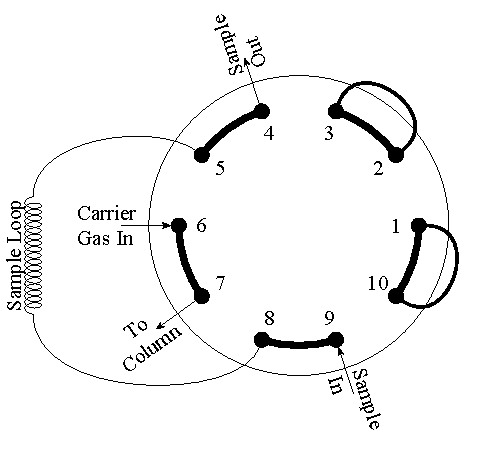
\includegraphics[width=7.9cm]{02-Experimental-Facilities/gcms-valve-load}}
                {\caption{Load position}
                \label{fig:gcms-valve-load}}
            \ffigbox[\FBwidth]
                {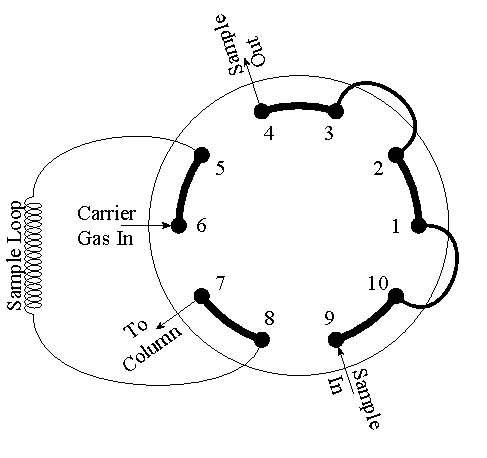
\includegraphics[width=7.9cm]{02-Experimental-Facilities/gcms-valve-inject}}
                {\caption{Inject position}
                \label{fig:gcms-valve-inject}}
        \end{subfloatrow}}
        {\caption{GC/MS sample injection valve.}
        \label{fig:gcms-valve}}
\end{figure}

\subsubsection{Mass Spectrometry}

Many types of detectors are available for GC analyses. These commonly include
flame ionization detectors, thermal conductivity detectors, and mass
spectrometers. In this work, a mass spectrometer is used to identify and
quantify the species eluted from the column.

The fundamental operation of a mass spectrometer (MS) is to detect the spectrum
of ions in a given sample. The MS generates this spectrum by detecting the
mass-to-charge ($m/z$) ratios of the ions. Ions are generated
from the effluent of the column---which includes sample components, mobile phase,
and column bleed, collectively called \textit{analytes}---by an ionization source,
typically either electronic or chemical in nature. Nearly all of the ions
generated will have a single charge, $z=1$ \cite{Sparkman2011}; thus,
the $m/z$ value of the ions is also equal to the mass of the ion.

In this work, electron ionization (EI) is used to generate the ions for
analysis. The effluent from the column is passed in front of an electron
source so that the electrons impact the analyte molecules and remove an
electron, generating a positive ion. EI is a \textit{hard ionization}
technique, in that the electron impact transfers a significant amount of energy
to the analyte molecule \cite{Sparkman2011}. The additional energy causes
the ion to fragment into two or more pieces; the spectrum of these fragments
is characteristic for a given molecule and can be used as a ``fingerprint''
to identify the source molecule for a given spectrum.

After ionization, the fragments are formed into a beam and accelerated out of the ionization
chamber towards the detector. Several detectors are available, including
time-of-flight and transmission quadrupole. All of these detectors require
high vacuum to avoid impact of the ion beam with extraneous species
prior to reaching the detector. The vacuum is achieved in the present
MS by a two-stage design, using a rotary vane pump in series with a
turbomolecular pump to achieve ultimate pressures of approximately \SI{2}{\pascal}.

\begin{figure}
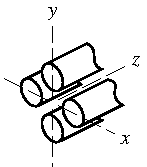
\includegraphics[width=7.9cm]{02-Experimental-Facilities/gcms-quad}
\caption{Schematic of the transmission quadrupole in an MS.}
\label{fig:gcms-quad}
\end{figure}

The MS used in this study is a transmission quadrupole type, shown
schematically in \cref{fig:gcms-quad}. The transmission quadrupole separates
specific ions from the ion beam by
means of a time-varying electric field. Conceptually, the quadrupole
can be imagined as four round rods, arranged in a cross pattern, with
their long axes aligned parallel to the ion beam (i.e. the $z$ axis).
The ions are admitted to the rods at one end (e.g. at the origin in
\cref{fig:gcms-quad}) and the detector is placed parallel to the $x-y$ plane
in \cref{fig:gcms-quad} at the other end of the rods(not shown in
\cref{fig:gcms-quad}). A positive DC voltage is applied
to one pair of the rods, while a negative DC voltage is applied to the other
pair of rods; in addition, an AC voltage is applied simultaneously to all four
rods. Assuming a specific ratio of AC amplitude to DC amplitude, ions of a certain
$m/z$ will remain in the ion beam and reach the detector.
Then, holding the AD:DC amplitude ratio fixed, the amplitudes are ramped with a known
function of time. This varies the particular $m/z$ that will remain in the ion beam
and reach the detector to be recorded \cite{Sparkman2011}, generating a mass spectrum.

The voltage amplitudes are ramped many times per second%
---typical ramp times range from \SIrange{0.05}{0.5}{\second},
depending on the range of $m/z$ values to be acquired---so that many
spectra are acquired during the elution of a given chemical compound
from the column, which typically occurs on the order of a few seconds.
For a given scan from the lowest to the highest amplitude, the number of ions
of each $m/z$ is measured at the detector. This information is
typically presented in the form of a relative intensity plot. The abscissa
is the (integer) $m/z$ while the ordinate is the intensity of a particular
$m/z$ scaled by the maximum intensity of all the $m/z$ in a given scan. It
is not required that the $m/z$ be integers, although they are usually presented
as such for simplicity. An example of a mass spectrum for a given time in a
GC/MS analysis is shown in \cref{fig:gcms-mass-spec}.

In addition to the mass spectrum, the MS reports the total ion current (TIC),
also known as the total ion chromatogram. This is the sum of all of the mass
intensities for a given scan. A sample TIC is plotted in \cref{fig:gcms-tic}
where the abscissa is time in \si{\minute} and the ordinate is an arbitrary unit.
Finally, the MS can also report the mass chromatogram (MC), which is the
chromatogram for a specific $m/z$ as a function of time.

\begin{figure}
    \begin{floatrow}
        \ffigbox
            {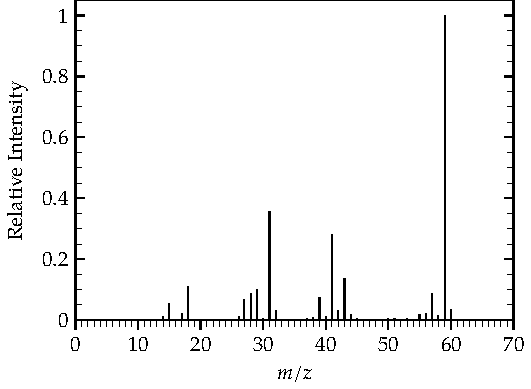
\includegraphics[width=7.9cm]{02-Experimental-Facilities/gcms-mass-spec}}
            {\caption{Example mass spectrum for a given scan during a GC/MS analysis}
            \label{fig:gcms-mass-spec}}
        \ffigbox
            {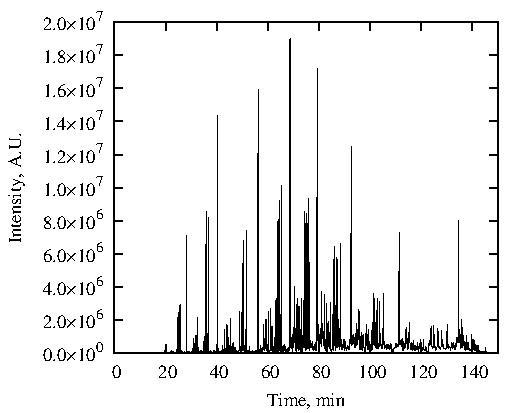
\includegraphics[width=7.9cm]{02-Experimental-Facilities/gcms-tic}}
            {\caption{Example TIC for a GC/MS analysis}
            \label{fig:gcms-tic}}
    \end{floatrow}
\end{figure}

\subsection{Identification and Quantification of Species using GC/MS}

Species are identified using a GC/MS system by their unique mass spectra.
Each peak in the TIC typically represents one compound eluting from the
column, although in theory each peak can represent more than one compound
if the compounds are retained similarly by the column. The peak is caused
by an increase in the number of ions reaching the detector on each scan
relative to the baseline as the compound elutes and is ionized. As
mentioned previously, many scans of the desired $m/z$ range are
conducted over the time that a compound is eluting from the column.
To determine the identity of a compound in a given peak, the set of
mass intensities over the peak are averaged and the background
spectrum is subtracted; this average spectrum is compared to a
database supplied by the National Institute of Standards and
Technologies (NIST). The database returns several suggested species
with a degree of matching parameter indicating how well the supplied
spectrum matches the spectrum in the database.

In this work, the external standard method of quantification is used.
This requires that calibration curves for each of the species of
interest be created, relating the area of the peak in the TIC to
the number of moles of analyte reaching the detector. The number of
moles of analyte can in turn be related to the number of moles of
sample in the gas sample injection valve sample loop. Once the
calibration curve is generated, it is used to relate the measured
area of the peak of particular component to its mole fraction. Detailed
methods for the construction of calibration curves will be given in
\cref{sec:gcms-procedure}.

\subsection{Experimental Procedure}
\label{sec:gcms-procedure}

The GC/MS used in this study is a
Shimadzu model QP-2010S, equipped with a 10-port Valco sample injection
valve and split/splitless injector, as mentioned previously. The column
used is a Phenomenex model ZB-5MS capillary column
with length \SI{30}{\meter}, inner diameter \SI{0.25}{\micro\meter}, and film
thickness of \SI{0.25}{\micro\meter}. The operating parameters of the GC/MS
(known as the ``method'') are shown in \cref{tab:gcms}.

The pressure in the gas injection valve sample loop is monitored by an
MMA type pressure transducer, the same model as used in \cref{sec:unc-p0}. The
sample outlet in \cref{fig:gcms-valve} is open to the atmosphere
so that a consistent pressure is maintained in the sample loop.
The volume of the sample loop is \SI{10}{\micro\liter}. With
the temperature, pressure, and volume of the sample loop known,
the number of moles of sample can be calculated by the ideal
gas law.

A calibration curve is built for the major species by the
following procedure. First, the sample bottle is vacuumed
to less than \SI{1}{\torr}. Mixtures of the species of
interest in the liquid state are prepared by massing each
component on a high-accuracy AND-201 scale. A small mass
of this mixture is drawn into a syringe and massed on the
same scale. The mixture is injected through a septum into
the sample bottle. Then the sample bottle is filled with
high-purity nitrogen so that the largest mole fraction of
a species of interest is approximately 0.001. The sample
bottle is connected to the sample injection valve on the
GC/MS and the valve on the sample bottle is opened and
quickly closed. The pressure is allowed to equalize and
the GC/MS is started.

After the completion of the GC/MS method, the total ion
chromatogram (TIC) is analyzed by the Shimadzu GCMS Post-run
Analysis software (version XXXX). Each peak is automatically
integrated by the software so that its area can be found.
The peak area is then related to the number of moles of
sample sent to the detector by linear least-squares regression.
This calibration curve is used to compute the mole fraction
of any given peak area for that species.

\end{document}
